\documentclass{article}
\usepackage[T1]{fontenc}
\usepackage{lmodern}
\usepackage[utf8]{inputenc}
\usepackage[british]{babel}
\usepackage{geometry}
\usepackage{color}
\usepackage{amsthm}
\usepackage{amsmath,amssymb}
\usepackage{graphicx}
\usepackage{mathtools}
\usepackage{listings}
\usepackage{newlfont}
\usepackage{tikz-cd}
\usepackage{rotating}
\usepackage[backend=biber]{biblatex}
\addbibresource{~/math/references.bib}

\newcommand{\numberset}{\mathbb}
\newcommand{\N}{\numberset{N}}
\newcommand{\Z}{\numberset{Z}}
\newcommand{\R}{\numberset{R}}
\newcommand{\Q}{\numberset{Q}}
\newcommand{\K}{\numberset{K}}
\newcommand{\F}{\numberset{F}}
\newcommand{\n}{\mathcal{N}}
\newcommand{\aid}{\mathfrak{a}}
\newcommand{\bid}{\mathfrak{b}}
\newcommand{\pid}{\mathfrak{p}}
\newcommand{\qid}{\mathfrak{q}}
\newcommand{\mi}{\mathfrak{m}}
\newcommand{\I}{\mathbb{I}}
\newcommand{\V}{\mathbb{V}}
\newcommand{\A}{\mathbb{A}}
\newcommand{\Ps}{\mathbb{P}}
\newcommand{\exercise}[1]{\noindent {\bf Exercise #1}}

\DeclareMathOperator{\Ima}{Im}
\DeclareMathOperator{\coker}{coker}
\DeclareMathOperator{\Id}{Id}
\DeclareMathOperator{\GL}{GL}
\DeclareMathOperator{\Mat}{Mat}
\DeclareMathOperator{\Ext}{Ext}
\DeclareMathOperator{\Tor}{Tor}
\DeclareMathOperator{\Hom}{Hom}

\begin{document}

\title{Algebraic Topology II - Assignment 2}

\author{Matteo Durante, s2303760, Leiden University}

\maketitle


~\\
\exercise{4}

\proof $(a)$ Consider the two open subsets of $SX$ given by $C_+X=X\times
(-1,1]_{/\sim},\ C_-X=X\times [-1,1)_{/\sim}$. We see that they are
contractible (we can collapse them to the pole they respectively contain) and
cover $SX$. By contractibility, $H^n(C_+X,R)\cong H^n(C_-X,R)
\cong 0$ for $n>0$.
\begin{align*}
    \cdots\rightarrow H^n(SX,C_+X;R)\rightarrow H^n(SX;R)\rightarrow
    H^n(C_+X;R)\rightarrow H^{n+1}(SX,C_+X;R)\rightarrow\cdots \\
    \cdots\rightarrow H^n(SX,C_-X;R)\rightarrow H^n(SX;R)\rightarrow
    H^n(C_-X;R)\rightarrow H^{n+1}(SX,C_-X;R)\rightarrow\cdots
\end{align*}
Looking at the long exact sequences of the pairs $(SX,C_+X),(SX,C_-X)$, since
$H^k(C_+X;R)\cong H^l(C_-X;R)\cong 0$, by exactness we can pull back the
elements $x,y$ to $x'\in H^k(SX,C_+X;R),y'\in H^l(SX,C_-X;R)$ respectively.

Consider the following diagram, where the homomorphism on the right is the
product of the ones of the previously mentioned long exact sequences (hence
$(x,y)$ is the image of $(x',y')$ under it), while the left one is the one in
long exact sequence of the pair $(SX,C_+X\cup C_-X)$:
\[
    \begin{tikzcd}
        H^k(SX,C_+X;R)\times H^l(SX,C_-X;R)\arrow{r}{-\cup -}\arrow{d}
        & H^{k+l}(SX,C_+X\cup C_-X;R)\arrow{d} \\
        H^k(SX;R)\times H^l(SX;R)\arrow{r}{-\cup -}
        & H^{k+l}(SX;R)
    \end{tikzcd}
\]

Notice that, since $C_+X\cup C_-X=SX$, the inclusion $C_+X\cup
C_-X\hookrightarrow SX$ induces for every $n$ isomorphisms $H^n(SX;R)\cong
H^n(C_+X\cup C_-X;R)$ in the long exact sequence of their
pair and therefore $H^{k+l}(SX,C_+X\cup C_-X;R)\cong 0$.

Since $C_+X$ and $C_-X$ are open subsets of $SX$, the (relative) cup product is
natural, the previous diagram commutes and then we have:
$$x\cup y=i^*_{C_+X}(x')\cup i^*_{C_-X}(y')=i^*_{C_+X\cup C_-X}(x'\cup y')=
i^*_{C_+X\cup C_-X}(0)=0\quad\square$$

~\\
\proof $(b)$ Let $x_i\in H^{k_i}(Y;R)$, $k_i>0$ for every $i$. Since for every $i$ we
have that $U_i\subset Y$ is contractible, $H^n(U_i;R)\cong 0$ for every $n>0$.
$$\cdots\rightarrow H^n(Y,U_i;R)\rightarrow H^n(Y;R)\rightarrow
H^n(U_i;R)\rightarrow H^{n+1}(Y,U_i;R)\rightarrow\cdots$$
Looking at the long exact sequences of the pairs $(Y,U_i)$, since
$H^{k_i}(U_i;R)\cong 0$ for every $i$, we can pull back each $x_i$ to some $x'_i
\in H^{k_i}(Y,U_i;R)$ by exactness.

Given $0<m<n$, we want to prove the commutativity of the following diagram and
to do so we will prove the commutativity of the one below, which is equivalent.
We understand $\Pi_{i=k}^n A_n$ to be $\cong 0$ when $k>n$, while the vertical
arrows are given by the products of the arrows (which we will denote by
$i^*_{\bigcup_{i=1}^m U_i}$ and $i^*_{U_i}$) of the long exact sequences of the
pairs $(Y,\bigcup_{i=1}^m U_i)$ and $(Y,U_i)$.
\[
    \begin{tikzcd}
        H^{\sum_{i=1}^m k_i}(Y,\bigcup_{i=1}^m U_i;R)\times\Pi_{i=m+1}^n
        H^{k_i}(Y,U_i;R)\arrow{r}{(-\cup-)\times\Id}\arrow{d}
        & H^{\sum_{i=1}^{m+1} k_i}(Y,\bigcup_{i=1}^{m+1}
        U_i;R)\times\Pi_{i=m+2}^n H^{k_i}(Y,U_i;R)\arrow{d} \\
        H^{\sum_{i=1}^m k_i}(Y;R)\times\Pi_{i=m+1}^n
        H^{k_i}(Y;R)\arrow{r}{(-\cup-)\times\Id}
        & H^{\sum_{i=1}^{m+1} k_i}(Y;R)\times\Pi_{i=m+2}^n H^{k_i}(Y;R) \\
        H^{\sum_{i=1}^m k_i}(Y,\bigcup_{i=1}^m U_i;R)\times
        H^{k_{m+1}}(Y,U_{m+1};R)\arrow{r}{-\cup-}\arrow{d}
        & H^{\sum_{i=1}^{m+1} k_i}(Y,\bigcup_{i=1}^{m+1} U_i;R)\arrow{d} \\
        H^{\sum_{i=1}^m k_i}(Y;R)\times H^{k_{m+1}}(Y;R)\arrow{r}{-\cup-}
        & H^{\sum_{i=1}^{m+1} k_i}(Y;R)
    \end{tikzcd}
\]
The commutativity of the latter diagram however is trivial, for again the $U_i$
are open subsets of $Y$, thus the (relative) cup product is a homomorphism which
is natural in this sequence. Now, by composing the horizontal arrows given by
the $(-\cup-)\times\Id$, we get the following commutative diagram:
\[
    \begin{tikzcd}
        \Pi_{i=1}^n
        H^{k_i}(Y,U_i;R)\arrow{rr}{-\cup\cdots\cup-}\arrow{d}{\Pi_{i=1}^n
        i^*_{U_i}}
        && H^{\sum_{i=1}^n k_i}(Y,\bigcup_{i=1}^n
        U_i;R)\arrow{d}{i^*_{\bigcup_{i=1}^n U_i}} \\
        \Pi_{i=1}^n H^{k_i}(Y;R)\arrow{rr}{-\cup\cdots\cup-}
        && H^{\sum_{i=1}^n k_i}(Y;R)
    \end{tikzcd}
\]
Notice that, since $\bigcup_{i=1}^n U_i=Y$, the inclusion $\bigcup_{i=1}^n
U_i\hookrightarrow Y$ induces for every $k$ isomorphisms $H^k(\bigcup_{i=1}^n
U_i;R)\cong H^k(Y;R)$ in the long exact sequence of the pair
$(Y,\bigcup_{i=1}^n U_i)$ and therefore $H^k(Y,\bigcup_{i=1}^n U_i;R)\cong 0$
for every $k$.

We also know that $(x_i)_{i=1}^n$ is the image of $(x'_i)_{i=1}^n$ under
$\Pi_{i=1}^n i^*_{U_i}$ by a previous observation.

It follows that:
$$x_1\cup\cdots\cup x_n=i^*_{U_1}(x'_1)\cup\cdots\cup
i^*_{U_n}(x'_n)=i^*_{\bigcup_{i=1}^n U_i}(x'_1\cup\cdots\cup
x'_n)=i^*_{\bigcup_{i=1}^n U_i}(0)=0\quad\square$$


~\\
\exercise{5}

Disclaimer: I have called $q$ the quotient map throughout the assignment by
mistake, leaving $f$ for the attaching maps of the 2-cells.

\proof $(a)$ We know that, up to homeomorphism, this space is the connected sum
of $g$ tori. We will therefore start computing the homology groups of this space.

We know that it is obtained as a $CW$-complex by taking one 0-cell
$e_0$, attaching to it $2g$ 1-cells $e^i_1$ through an attaching map $g$ and
finally attaching to these
1-cells a 2-cell $e_2$, where the attaching map $f$ starts from $e_0$, runs
through $e^1_1,e^2_1,e^{-1}_1,e^{-2}_1,e^3_1,e^4_1,e^{-3}_1,e^{-4}_1,e^5_1$ and
so on, until it has run through $e^{-2g}_1$. By $e^{-i}_1$ we denote the cell
$e^i_1$ with opposite orientation.
 
We know that the (relevant section of the) cellular chain complex is given by:
$$0\rightarrow\Z\rightarrow\Z^{2g}\rightarrow\Z\rightarrow 0$$

At all of the other levels we have 0.

We proceed now to compute the homology groups of our surface, which coincide with
the ones of the homology groups of this chain complex.

Clearly, for every $n>2$ we have that $H_n(\Sigma_g)\cong 0$.

Consider now the generating element of $\Z^{2g}$ associated to the 1-cell
$e^1_i$. We will prove that it is mapped to 0 by computing the
mapping degree of the following composite:
$$\partial D^1\xrightarrow{l|_{\partial
D^1_i}} X_0\xrightarrow{q} X_0/X_{-1}\xrightarrow{q'}
D^0/\partial D^0\xrightarrow{h_0}\partial D^1$$

We see that, since $X_0=\{e_0\}$, this map is constant for every $i$, hence the
mapping degrees are always 0 and therefore the homomorphism $\Z^{2g}\rightarrow
\Z$ is the zero homomorphism as well.

It follows that $H_0(\Sigma_g)\cong\Z$.

Continuing, we show that the map $\Z\rightarrow\Z^{2g}$ is again zero in the
same way, i.e. by computing the mapping degree of the following composites:
$$\partial D^2\xrightarrow{f} X_1\xrightarrow{q} X_1/X_0\xrightarrow{q_i}
D^1/\partial D^1\xrightarrow{h_1}\partial D^2$$

We see that $f$ sends the loop given by $\partial D^2$ to the loop
described by the attaching map $f$, then $q$ does not act, while $q_i$ collapses
all of the cells different from $e^i_1$ to $e_0$, thus leaving only a
loop wrapping $e^i_1$ first in one direction and then in the other. This loop
can therefore be contracted to a constant one, hence the composite map is again
homotopic to a constant map and its mapping degree is 0 for every $i$.

Since this is a zero map, we have that
$H_1(\Sigma_g)\cong\Z^{2g},H_2(\Sigma_g)\cong\Z$.

All of these homology groups are free $\Z$-modules, hence we have that
$\Ext^1_{\Z}(H_n(\Sigma_g),\Z)\cong 0$ for every $n$. It follows from the
universal coefficient theorem that
$H^n(\Sigma_g)\cong\Hom_{\Z}(H_n(\Sigma_g),\Z)\cong H_n(\Sigma_g)$ for every
$n$ under the isomorphism given by $f\mapsto (f(v_i))_{i\in I}$, where the $v_i$
form the canonical basis of $H_n(\Sigma_G)$.$\quad\square$

~\\
\proof $(b)$ Consider a point $O$ in the interior of the cell $e_2$ and then
draw within the cell the segments from the meeting point of $e_1^{-2i}$ and
$e_1^{2i+1}$ or $e^{-2g}_1$ and $e^1_1$ to
it (see the picture in the next page for added clarity: these points are
actually identified and therefore there is ambiguity). We see that, by
identifying the points of $\Sigma_g$ in these segments,
we get a space homeomorphic to $\vee_g\Sigma_1$ since $\Sigma_{g/\sim}$ can be
represented as $g$ squares with the edges identified as they would be in a torus
and having identified vertices.
\begin{figure}[h!]
    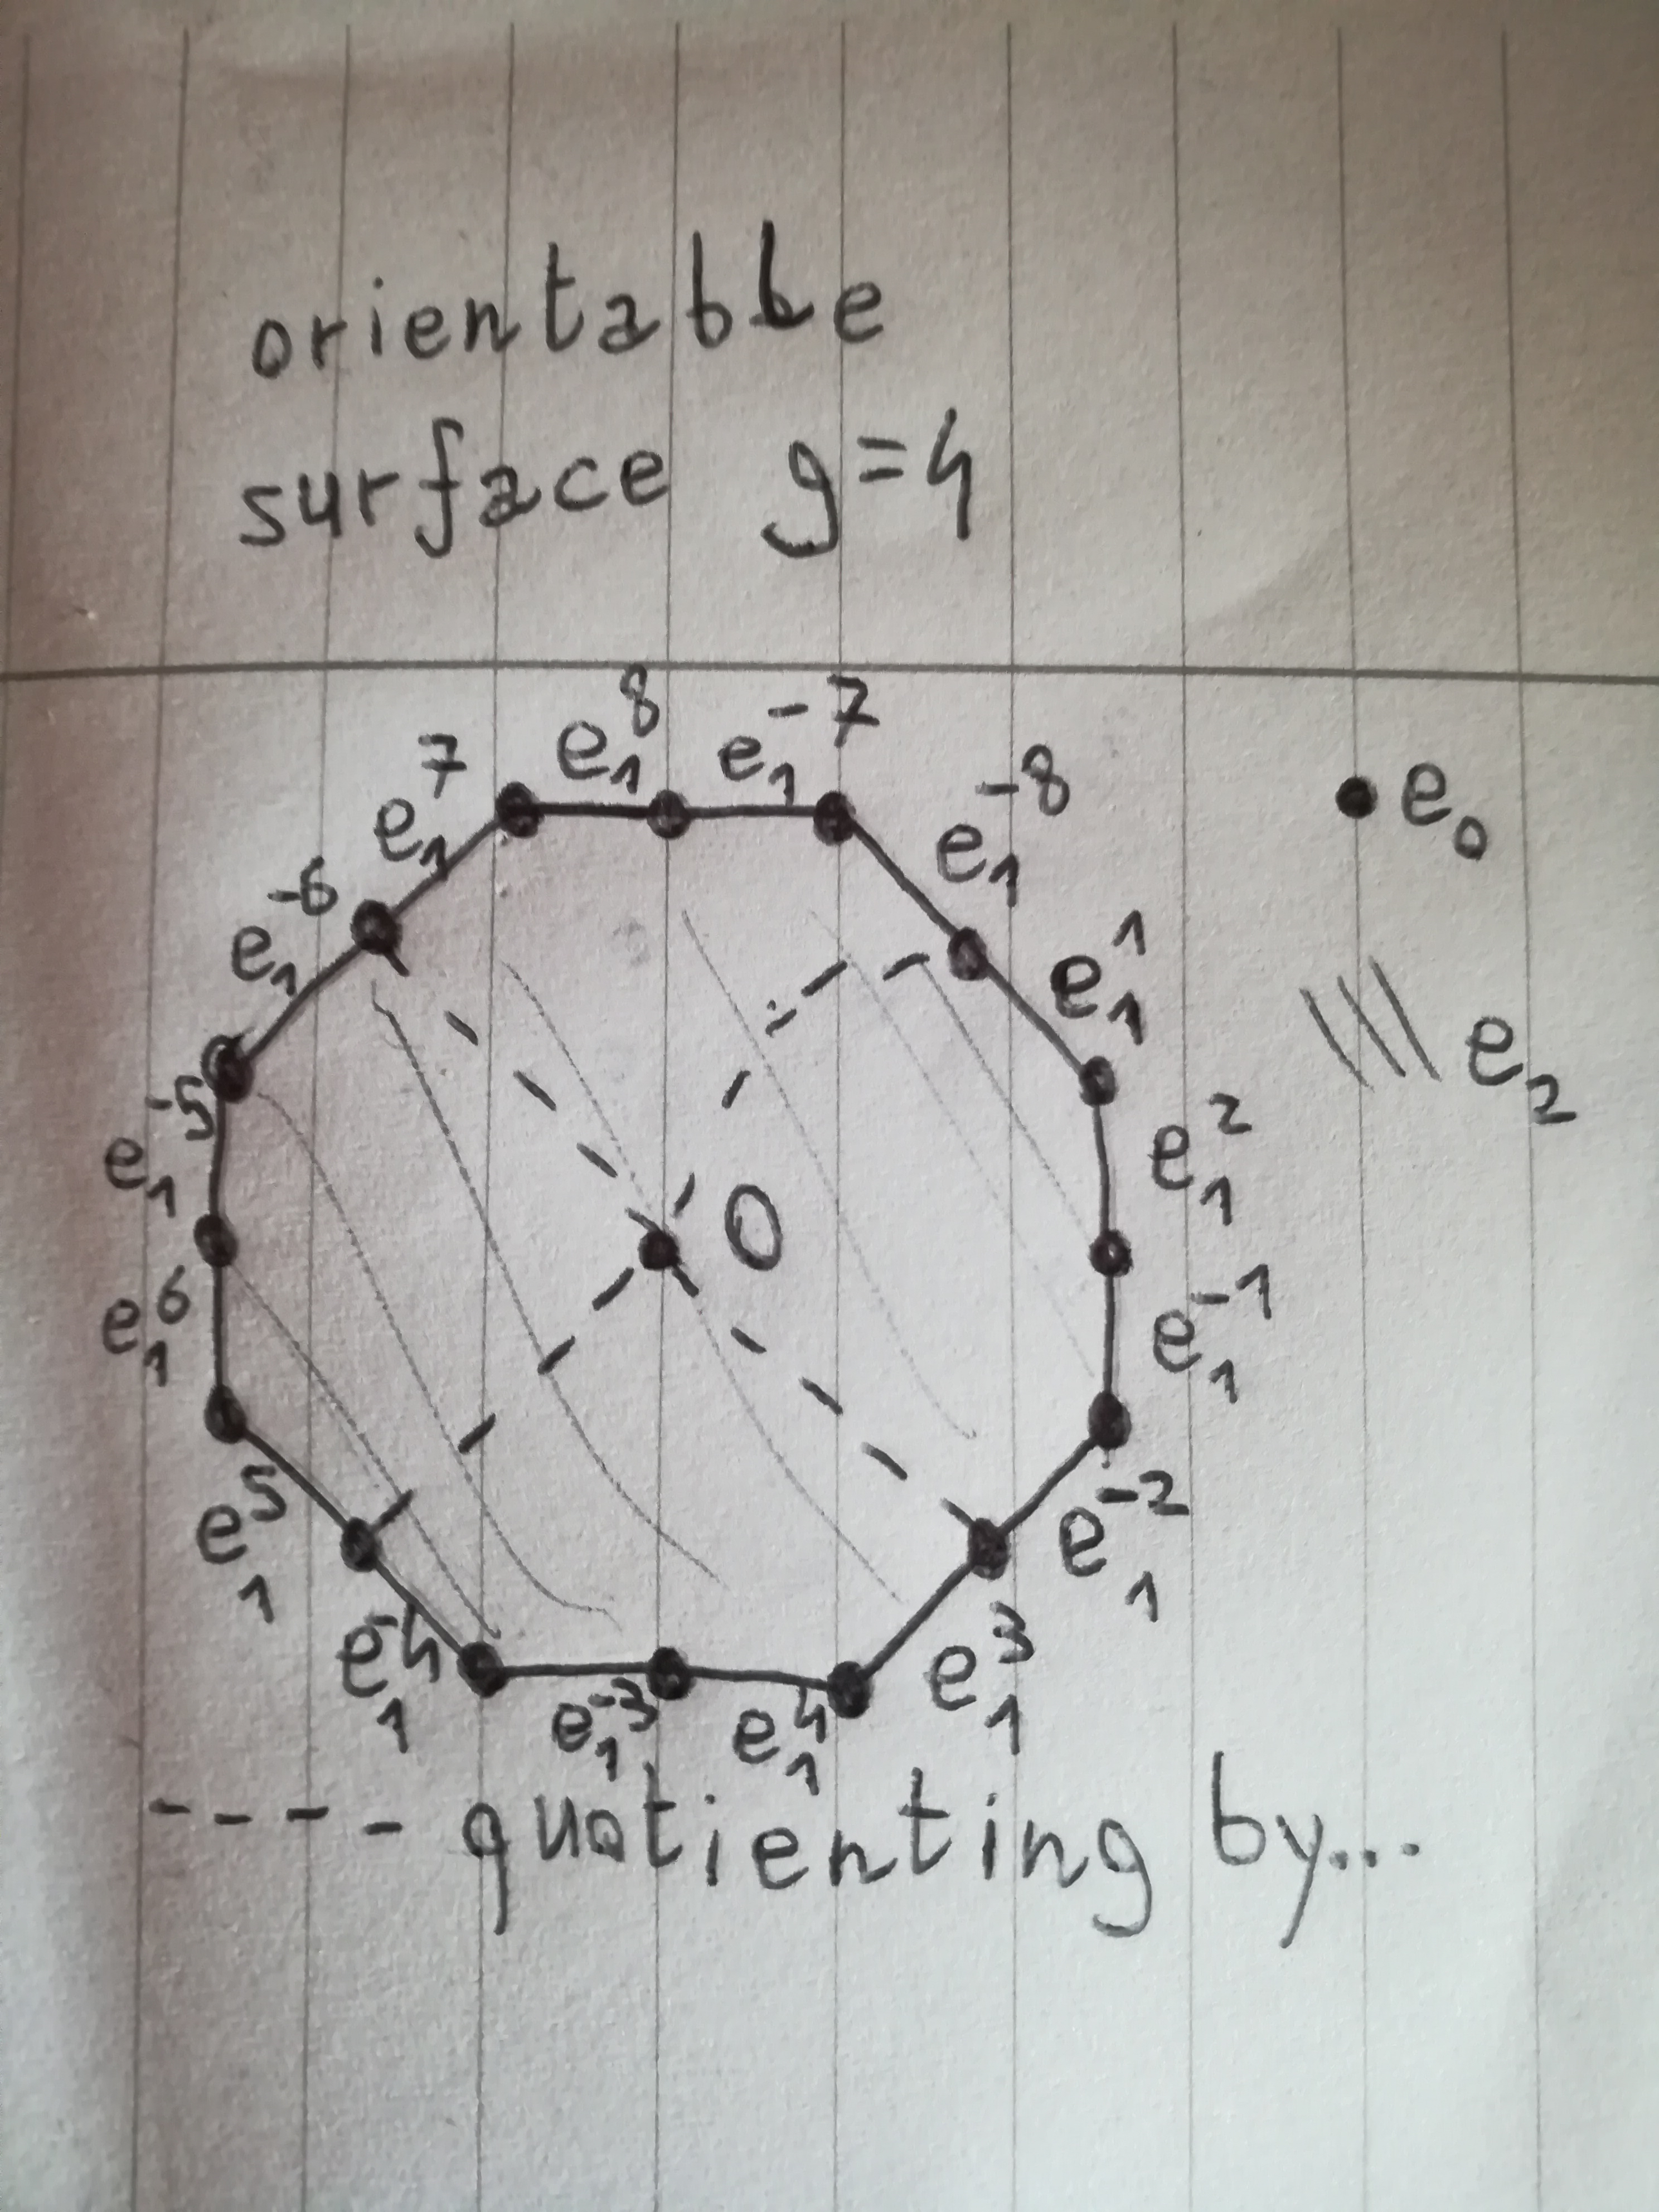
\includegraphics[width=5cm]{IMG_20190307_130206.jpg}
\end{figure}

We will consider the map $\Sigma_g\xrightarrow{q}\vee_g\Sigma_1$ induced by the
quotient.

Under this map, the $(2i+j)$th 1-cell
($i\in\{0,\ldots,g-1\},j\in\{1,2\}$) is sent to the $j$th
1-cell of the $i$th torus.

We know that $\vee_g\Sigma_1$ can be obtained by taking a
0-cell $e_0$, attaching to it $2g$ 1-cells $e_1^i$ using the attaching map $l$ 
and then attaching $g$
2-cells $e_2^j$, where the attaching map $f$ sends the $j$th $\partial D^2$ to a loop
starting in $e_0$ and running through the 1-cells $e_1^j,e_1^{j+1},e_1^{-j}$ and
finally $e_1^{-(j+1)}$.

Here, the cellular chain complex is given by:
$$0\rightarrow\Z^g\rightarrow\Z^{2g}\rightarrow\Z\rightarrow 0$$

Now we compute $H_n(\vee_g\Sigma_1)$.

Again, for $n>2$ we have trivially that $H_n(\vee_g\Sigma_1)\cong 0$.

Like before, we study the group homomorphism $\Z^{2g}\rightarrow\Z$ by computing
the mapping degrees of the following composites:
$$\partial D^1\xrightarrow{l|_{\partial
D^1_i}} X_0\xrightarrow{q} X_0/X_{-1}\xrightarrow{q'}
D^0/\partial D^0\xrightarrow{h_0}\partial D^1$$

Like before, since $X_0=\{e_0\}$ the composite is constant, thus its mapping
degree is 0 for every $i$. It follows that this is the zero map.

We do the same with $\Z^g\rightarrow\Z^{2g}$:
$$\partial D^2\xrightarrow{f|_{\partial D^2_j}} X_1\xrightarrow{q} X_1/X_0
\xrightarrow{q_i} D^1/\partial D^1\xrightarrow{h_1}\partial D^2$$

Like before, the loop $\partial D^2$ is sent to the loop earlier described to
attach the $j$th cell to $X_1$, while $q'$ does not act and $q_i$ collapses
every 1-cell distinct from $e^i_1$ to $e_0$. If $i\neq 2j-1,2j$, then the loop
we get is constant, hence the composite is a constant map, otherwise we get a
loop running through $e^i_1$ and then $e^{-i}_1$, thus it can be contracted to a
constant one and the composite map is homotopic to a constant map, thus the
mapping degree is again 0.

It follows that $H_1(\vee_g\Sigma_1)\cong\Z^{2g},H_2(\vee_g\Sigma_1)\cong\Z^g$.

Again, since all of these homology groups are free $\Z$-modules and therefore
$\Ext^1_{\Z}(H^n(\vee_g\Sigma_1),\Z)\cong 0$, by the
universal coefficient theorem we deduce that
$H^n(\vee_g\Sigma_1)\cong\Hom_{\Z}(H_n(\vee_g\Sigma_1),\Z)\cong
H_n(\vee_g\Sigma_1)$.

We are about to show that $H_1(\Sigma_g)\xrightarrow{q_*}H_1(\vee_g\Sigma_1)$
is an isomorphism.

Let's look at the map of cellular chain complexes induced by $q$. If we can
prove that it defines an isomorphism between the two $\Z^{2g}$
then we are done since it will induce the same map on the homology groups.
\[
    \begin{tikzcd}
        0\arrow{r} &\Z\arrow{d}{q_*}\arrow{r}
        &\Z^{2g}\arrow{d}{q_*}\arrow{r} &\Z\arrow{d}{q_*}\arrow{r} &0 \\
        0\arrow{r} &\Z^g\arrow{r} &\Z^{2g}\arrow{r} &\Z\arrow{r} &0
    \end{tikzcd}
\]
We know that $\Z^{2g}$ has a canonical basis of $2g$ elements, the
$(\delta_{i,j})_{j=1}^{2g}$ with $i\in\{1,\ldots 2g\}$, where the $i$th
generator describes a loop running through the $i$th 1-cell only once.
Under the quotient map, the loop related
to the $i$th 1-cell is sent to the loop in $\vee_g\Sigma_1$ running through the
$i$th 1-cell only once, which corresponds again in the group $\Z^{2g}$ of the
lower chain to the element written as $(\delta_{i,j})_{j=1}^{2g}$. Since $q_*$
acts as the identity map on
the generators, it acts as the identity map overall and we are done.

Now we prove that $q^*$ is an isomorphism as well.

Consider the following morphism between the exact sequences described by the
universal coefficient theorem:
\[
    \begin{tikzcd}
        0\arrow{r} &\Ext^1_{\Z}(H_1(\vee_g\Sigma_1),\Z)\cong
        0\arrow{r}\arrow{d}{\Ext^1_{\Z}(q_*,\Z)}
        &H^1(\vee_g\Sigma_1)\arrow{r}{\sim}\arrow{d}{q^*}
        &\Hom_{\Z}(H_1(\vee_g\Sigma_1),\Z)\arrow{r}\arrow{d}{\Hom_{\Z}(q_*,\Z)} &0 \\
        0\arrow{r} &\Ext^1_{\Z}(H_1(\Sigma_g),\Z)\cong 0\arrow{r}
        &H^1(\Sigma_g)\arrow{r}{\sim} &\Hom_{\Z}(H_1(\Sigma_g),\Z)\arrow{r} &0 \\
    \end{tikzcd}
\]
Since $q_*$ is an isomorphism, $\Hom_{\Z}(q_*,\Z)$ is an isomorphism as well and
therefore the same goes for $q^*$, which is its dual (just like the cohomology
groups in this case are the duals of the homology groups, even though this is
true for every $n$). Also, since the
universal coefficient theorem is natural, the diagram shows that $q^*$ maps
generators to generators in the natural way, that is
$\alpha_i\mapsto\alpha_i,\beta_i\mapsto\beta_i$.$\quad\square$

~\\
\proof $(c)$ We want to give a description of the map $q_*$ on the $H^2$.

Pick a point $x\in\Sigma_g$ in the interior of the 2-cell s.t. $q(x)$ is not
the base point of $\vee_g\Sigma_1$. We see that $\Sigma_g\setminus\{x\}$ can be
retracted to the 1-cells and hence it is homotopy equivalent to $\vee_g S^1$, a
CW-complex of dimension 1.

It follows that $H_2(\Sigma_g\setminus\{x\})\cong
H_3(\Sigma_g\setminus\{x\})\cong 0$.

Let's keep in mind the following diagram, where the vertical maps are given by the
long exact sequences of their respective pairs:
\[
    \begin{tikzcd}
        H_2(\Sigma_g)\arrow{r}{q_*}\arrow{d}{\sim} 
        &H_2(\vee_g\Sigma_1)\arrow{d} \\
        H_2(\Sigma_g,\Sigma_g\setminus\{x\})\arrow{r}{q_*}
        &H_2(\vee_g\Sigma_1,\vee_g\Sigma_1\setminus\{q(x)\})
    \end{tikzcd}
\]

If $q(x)$ lies in the $i$th torus, we have that
$H_2(\vee_g\Sigma_1,\vee_g\Sigma_1\setminus\{q(x)\})\cong
\tilde{H}_2(\vee_g\Sigma_1/\vee_g\Sigma_1\setminus\{q(x)\})\cong
\tilde{H}_2(\Sigma^i_1/\Sigma^i_1\setminus\{q(x)\})\cong
H_2(\Sigma^i_1,\Sigma^i_1\setminus\{q(x)\})\cong\Z$ (*), which is generated by the image of
$c_i$, the generator of $H_2(\vee_g\Sigma_1)$ associated to the $i$th 2-cell (to
see why, observe that $H_3(\vee_g\Sigma_1\setminus\{q(x)\})\cong 0$ by a similar
reasoning as the one presented in (*), thus the map 
$H_2(\vee_g\Sigma_1)\rightarrow
H_2(\vee_g\Sigma_1,\vee_g\Sigma_1\setminus\{q(x)\})$ must be surjective).

Also, $q$ is locally at $x$ an homeomorphism, thus it sends a generator of
$H_2(\Sigma_g,\Sigma_g\setminus\{x\})$ to a generator of
$H_2(\vee_g\Sigma_1,\vee_g\Sigma_1\setminus\{q(x)\})$

Notice that $x$ can be chosen such that $q(x)$ lands in any torus of
$\vee_g\Sigma_1$, hence,
looking at our diagram, the generator $c$ of $H_2(\Sigma_g)$ is sent by $q_*$ to a sum
$\sum_g\pm c_i$, where all of the
signs can be positive if we choose our generators correctly.

(*) Indeed, again $\Sigma_1\setminus\{q(x)\}$ is homotopy equivalent to $\vee_2 S^1$
by rectracting it to its 1-cells and $H_2(\vee_2 S^1)\cong H_3(\vee_2 S^1)\cong
0$. Now look at the long exact sequence of the pair
$(\Sigma_1,\Sigma_1\setminus\{q(x)\})$, which with our previous observations tells us that
$H_2(\vee_g\Sigma_1,\vee_g\Sigma_1\setminus\{q(x)\})\cong H_2(\Sigma_1)\cong\Z$.

Now, let's call $a_i,b_i$ the generators of $\Sigma_g$ associated to the $i$th
cell, $\alpha_i,\beta_i$ their duals. Likewise, the dual of $c$ will be
$\sigma$.

Let's focus on the following commutative diagram:
\[
    \begin{tikzcd}
        H^1(\vee_g\Sigma_1)\times
        H^1(\vee_g\Sigma_1)\arrow{d}{q^*}\arrow{r}{-\cup-}
        & H^2(\vee_g\Sigma_1)\arrow{d}{q^*} \\
        H^1(\Sigma_g)\times H^1(\Sigma_g)\arrow{r}{-\cup-}
        & H^2(\Sigma_g)
    \end{tikzcd}
\]

We see that we can pull back the $\alpha_i$ and $\beta_i$, do the computations
in $H^*(\vee_g\Sigma_1)$ and then push forward the result in $H^*(\Sigma_g)$ by
making use of the naturality of the cup product and the fact that $q^*$ is a
ring homomorphism.

Pulling them back, we will get the generators $\alpha$ ($i$th torus) and $\beta$
($i$th torus).

Now we want to prove that, for $i\neq j$,
$\alpha_i\cup\alpha_j=\alpha_i\cup\beta_j=\beta_i\cup\beta_j=0$.

Consider two non-zero elements $d,d'$ related to two different tori. We may
assume that they are preimages of some ($\alpha_i$ or $\beta_i$) and
($\alpha_j$ or $\beta_j$) respectively, $i\neq j$. We can draw
the following diagram, where the vertical arrows are given by the exact
sequences of the obvious pairs:
\[
    \begin{tikzcd}
        H^1(\vee_g\Sigma_1,(\Sigma^i_1)^c\cup\{q(x)\})\times
        H^1(\vee_g\Sigma_1,\Sigma^i_1)\arrow{d}\arrow{r}{-\cup-}
        & H^2(\vee_g\Sigma_1,(\Sigma^i_1)^c\cup\Sigma^i_1)\arrow{d} \\
        H^1(\vee_g\Sigma_1)\times H^1(\vee_g\Sigma_1)\arrow{r}{-\cup-}
        & H^2(\vee_g\Sigma_1)
    \end{tikzcd}
\]

Now, since $H^2(\vee_g\Sigma_1,(\Sigma^i_1)^c\cup\Sigma_i)\cong
H^2(\vee_g\Sigma_1,\vee_g\Sigma_1)\cong 0$, remembering that the diagram
commutes by the naturality of the (relative) cup product over subcomplexes
and being able to pull back $d$ to $H^1(\vee_g\Sigma_1,(\Sigma^i_1)^c\cup\{q(x)\})$, $d'$ to
$H^1(\vee_g\Sigma_1,\Sigma^i_1)$, we can conclude that $d\cup d'=0$.

From this it follows that
$\alpha_i\cup\alpha_j=\alpha_i\cup\beta_j=\beta_i\cup\beta_j=0$ for $i\neq j$ in
$H^*(\Sigma_g)$.

Consider now the following diagram, where the (relative) cup product is natural
because $\Sigma^i_1$ is closed in $\vee_g\Sigma_1$:
\[
    \begin{tikzcd}
        H^1(\vee_g\Sigma_1,(\Sigma^i_1)^c)\times
        H^1(\vee_g\Sigma_1,(\Sigma^i_1)^c)\arrow{d}\arrow{r}{-\cup-}
        & H^2(\vee_g\Sigma_1,(\Sigma^i_1)^c)\arrow{d} \\
        H^1(\vee_g\Sigma_1)\times H^1(\vee_g\Sigma_1)\arrow{r}{-\cup-}
        & H^2(\vee_g\Sigma_1)
    \end{tikzcd}
\]

We will prove that $\alpha_i\cup\beta_i=\sigma$ in $H^*(\Sigma_g)$.

Now, notice that we can pull back the preimages of $\alpha_i,\beta_i$ (which we
will call with the same names) to $H^1(\vee_g\Sigma_1,(\Sigma_1)^c)$. Observing
that $H^n(\vee_g\Sigma_1,(\Sigma^i_1)^c)\cong
\tilde{H}^n(\vee_g\Sigma_1/(\Sigma^i_1)^c)\cong\tilde{H}^n(\Sigma^i_1)\cong
H^n(\Sigma^i_1,*)\cong H^n(\Sigma^i_1)$ naturally for $n>0$, we can carry out
the computations in $H^*(\Sigma^i_1)$ and then push the result forward in
$H^2(\vee_g\Sigma_1)$.

Since in $H^*(\Sigma_1)$ we have (up to sign) that $\alpha\cup\beta=\sigma$, we get that
$\alpha_i\cup\beta_i=\sigma_i$ in $H^*(\vee_g\Sigma_1)$, which then under the
dual map $q^*$ is sent to $\sigma$ (remember that at this level $q^*$ is the
dual of $c\mapsto\sum_g c_i$, $c$ and
$\{c_i\}_{i=1}^g$ being systems of generators of the respective homology groups),
thus $\alpha_i\cup\beta_i=\sigma$ in $H^*(\Sigma_g)$.

In the same way we get that $\alpha_i\cup\alpha_i=0,\beta_i\cup\beta_i=0$,
thus we can conclude.$\quad\square$

\printbibliography

\end{document}


